\documentclass[a4paper, 12pt]{./Template/lnls-note}
\usepackage{amsmath}
\usepackage{amssymb}
\usepackage{amsthm}
\usepackage{indentfirst}
\numberwithin{equation}{section} %enumerate equations acording to their sections
\usepackage[pdftex,colorlinks=true,citecolor=black,linkcolor=black,urlcolor=black,filecolor=black]{hyperref}
\usepackage[num,abnt-emphasize=bf, bibjustif]{abntex2cite}
\usepackage{tipa}
\usepackage{ulem}
\usepackage{mathrsfs}
\citebrackets[]
%\documentclass[a4paper, 12pt, report]{lnls-note} % if you want to have chapters choose this one
\newcommand*\blankpage{\newpage\null\thispagestyle{empty}\newpage}
%loads standard preamble configuration
%Standard preamble for documentation preparation

% \usepackage[T1]{fontenc}
% \usepackage{txfonts}
% \usepackage{authblk} % para varios autores em um mesmo artigo
\usepackage{graphicx}
\usepackage{subfigure}
\usepackage{fancyvrb} %fancy verbatim environment
\usepackage{amssymb}  % more symbols
% \usepackage{booktabs}
\usepackage{multirow} % enable multi row in tables
\usepackage{ulem}  % used to strike text
\usepackage{scrextend} % allow reference to footnotes
\usepackage[version=3]{mhchem} % Package for chemical equation typesetting
\usepackage{siunitx} % Package for units in SI
\usepackage{amsmath} % package with several mathematical symbols
% \usepackage{mathtools} % aligned environment inside align environment
% \usepackage[num]{abntcite}
\usepackage{lmodern} % carrega a fonte natural do latex com T1
\usepackage{textcomp} % package with symbols
\usepackage{floatrow}% Table float box with bottom caption, box width adjusted to content
\usepackage[hang,small]{caption}% legendas menores e o hang=alinha a legenda
\usepackage{hyperref} %possibilita o uso das refer�ncias e hiperlinks
\hypersetup{colorlinks,%
	    citecolor=black,%
	    filecolor=black,%
	    linkcolor=black,%
	    urlcolor=blue}
\usepackage{algpseudocode} %algorithmic package
\usepackage{algorithm}     % float environment for algorithm

%loads standard commands
\newcommand{\mc}[3]{\multicolumn{#1}{#2}{#3}} % multicolumns in a table
\newcommand{\mr}[3]{\multirow{#1}{#2}{#3}}    % multirows in a table
\newcommand{\deriva}[2]{\frac{\text{d} #1}{\text{d} #2}} % derivada de #1 em relacao a #2
\newcommand{\bit}{\begin{itemize}}
\newcommand{\eit}{\end{itemize}}
\newcommand{\bce}{\begin{center}}
\newcommand{\ece}{\end{center}}
\newcommand{\beq}{\begin{equation}}
\newcommand{\eeq}{\end{equation}}
\newcommand{\bfl}{\begin{flushleft}}
\newcommand{\efl}{\end{flushleft}}
\newcommand{\degre}{$^\circ$}% Changed this one because there already is a \degree macro in latex
\newcommand{\see}{$\rightarrow$}
\newcommand{\nmrad}{nm$\cdot$rad}
\newcommand{\powten}[1]{$\cdot 10^{#1}$}

\newcommand{\frage}[1]{~\\ \fbox{\small \tt #1}\\}




\begin{document}

\lnlstitle{134518}{\today}{Tune Measurement and Correction Systems}
{Isabella Stevani}{\LNLS}
{This document contains information about discussions and experiments done about tune measurement and correction systems. Its intention is to help in the comprehension about these two systems, using as an example the systems from UVX, the current operating particle accelerator at the Brazilian Synchrotron Light Laboratory (LNLS).}

\blankpage
\newpage
\tableofcontents
\thispagestyle{empty}
\blankpage

\newpage
\setcounter{page}{5}
\section{Systems}
	\subsection{Signal analyzer system}
This is a \textbf{measurement} system.

The measurement is done by a signal analyser operating in spectrum mode. Its OUT pin is connected to an amplifier, which is connected to one of the eight connectors available on a stripline. The signal generated by the signal analyzer is a sinusoid with fixed amplitude and variable frequency (generally, this variation follows a sawtooth function).

\begin{itemize}
	\item An amplifier is needed because the signal from the signal analyzer has not enough power to excite the beam.
	\item The opposite connector of the stripline is connected with an 50$\Omega$ load so the excess power could dissipate (the beam absorb only a few percent of the excitation power).
	\item To determinate the frequency range of the excitation signal, an initial and a final frequencies should be define. For tune measurement application, those two frequencies should be chosen in a way that the range contains the horizontal and vertical betatron frequencies.
	\item The amplifier gain could be adjusted remotely, but this is not considered in the measurement loop yet.
\end{itemize}

The signal received by the stripline excites the beam over a predefined frequency range. But is known that the beam oscillation amplitudes grow at the betatron frequencies, so its frequency response should be something like \autoref{fig:signalanalyzer_frequencyresponse}.

\begin{figure}[!htb]
	\centering
	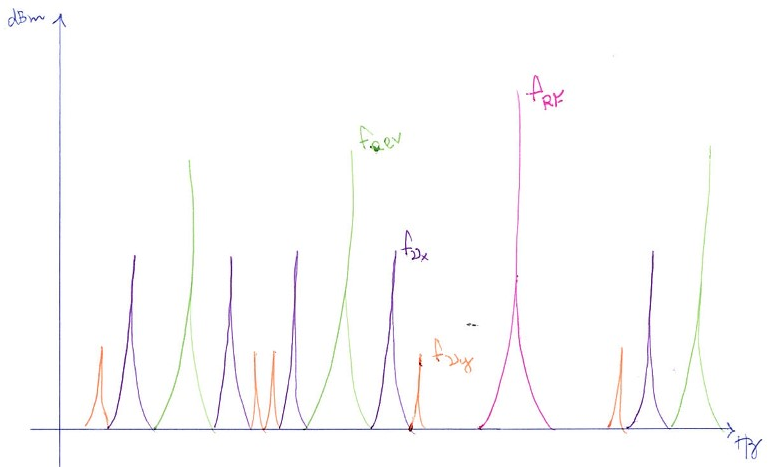
\includegraphics[width=0.9\linewidth]{./Figures/signalanalyzer_frequencyresponse.png}
	\caption{Rough sketch of the beam oscillation frequency response.}
	\label{fig:signalanalyzer_frequencyresponse}
\end{figure}

The tunes can be obtained by the distance between the betatron frequencies ($f_{\nu_x}$ e $f_{\nu_y}$) and their respective revolution harmonic. Dividing that distance by the revolution frequency, you can obtain the tune fractional part.

The beam oscillations are measured by a beam position monitor (BPM), stripline type. One of its connections is connected to the OUT pin of the signal analyzer.

\begin{itemize}
	\item On both excitation and measurement processes, only one antenna is used. This configuration is sufficient because the antennas inside the striplines are positioned across de major axis (in other words, they're positioned like an X over tha vacuum chamber) in a way that its signal contains both plane information.
	\item The fact mentioned above is only possible because the bean trajectory oscillations (the ones caused by the betatron and dispersion functions) occurs in a frequency much smaller than the excitation range of frequencies. Regarding that the excitation signal comes from the signal analyzer, this one knows exactly in which frequency it should analyze the signal, so it filters the measurement only over the predefined frequency range. In other cases, would be necessary collect the measurement from two opposite antennas and subtract their signals to obtain information only from the excitation oscillations.
\end{itemize}

\subsubsection{Notes}
It's important to emphasize one characteristic of this system. The excitation signal excites \textbf{all bunches}, no exception. But the power absorbed by them is so little that this don't affect the beam dynamics in a significant proportion. Still, it's sufficient to compute the tune measurement due to the great sensibility of the signal analyzer.

\subsubsection{Possible issues and solutions}
\noindent
\textbf{Plane identification}\\

The signal analyzer system from UVX works with both planes at the same time, so both x-axis and y-axis frequency responses are displayed on the screen together. In that configuration, sometimes could be difficult for the tune measurement algorithm to identify which peak belongs to which axis.

A possible solution to that would be working with each plane separately, exciting and measuring one plane at a time with a switch to do that shift. The benefits would be that x-axis and y-axis measurements would be more isolated from each other, but the shifting process would make impossible to measure both planes simultaneously like the actual system does. Also, the measurement process would became slower.\\ \\

\noindent
\textbf{Peak tracking when operating with low-current}\\

When the machine is operating with low-current, the beam frequency response generated by the excitation process could be so small that, if the tune measurement algorithm is based on a peak tracking logic, it could not be able to distinguish the right peak from noise.

A way to increase the frequency response amplitude is to increase the amplifier gain, transferring more energy to the beam during the excitation process. So, a good solution to this problem would be adding the amplifier gain in a control loop that identifies if the machine is operating with low-current. If it is, the amplifier gain is increased to make the tune measurement possible.

\pagebreak
	\subsection{UVX devices}
Here are described some characteristics of the devices from UVX used in any of the systems presented in this document.

\subsubsection{Signal analyzer system}

\begin{itemize}
	\item \textbf{Excitation device}\\
		Device: Stripline\\
		Name: AEX08\\
		Available connectors: 8\\
		Length: 15 cm
	\item \textbf{Measurement device}\\
		Device: BPM Stripline type\\
		Name: AMP11B\\
		Available connectors: 4 (4 others internally short-circuited)\\
		Length: 6 cm
\end{itemize}

\newpage
\bibliography{biblio}


\end{document}








